
\chapter[ಭಾಗ -  2]{}\label{chap2}

\begin{center}
\rule{5cm}{1pt}\\[5pt]
{\Large\bfseries ಅಲಂಕಾರಿಕ ವಸ್ತುಗಳ ತಯಾರಿಕೆ }\\[3pt]
\rule{5cm}{1pt}
\end{center}
 
 \begin{itemize}
 \item ನಿರ್ದಿಷ್ಟ ಮಾನ ಆಕಾರಗಳು (6 ರೀತಿಯಲ್ಲಿ)
 \item  ಮೀನನ ರಚನೆ
 \item Flower for Rose
 \item Six point star
 \item ಮಾಘ ಮಾಲೆ
 \item ಹಡಗ ತಯಾರಿಕೆ
 \item ದ್ವಿಪಾದ ಹಡಗು
 \item wind mill
 \item ಟ್ರೇ
 \item ಕಪ್ 
 \item samurais Helmet
 \item  yakka-San.
  \end{itemize}
 
 \section*{ಓರಿಗಾಮಿಯಲ್ಲಿ ನಿರ್ದಿಷ್ಟ ಮಾನ ಆಕಾರಗಳು [Standard Shapes]}
 
 ಈಗ ಸಾವಿರಾರು ಕಾಗದದ ಮಾದರಿಗಳನ್ನು ತಯಾರಿಸುವುದನ್ನು ತಿಳಿದುಕೊಂಡಿದ್ದೇವೆ. ಈ ಕಾಗದ ಮಾದರಿಗಳನ್ನು ತಯಾರಿಸುವಾಗ ಅನೇಕ ಹಂತಗಳಲ್ಲಿ ಕಾಗದವನ್ನು ಮಡಚಬೇಕಾಗುತ್ತದೆ. ಹೀಗೆ ಮಡಚಬೇಕಾದರೆ, ಒಂದು ನಿರ್ದಿಷ್ಟ ಆಕಾರದ ಮಡಚುವಿಕೆಯನ್ನು ಪ್ರಾರಂಭದ ಹಂತದಲ್ಲಿ ಬಳಸುತೇವೆ. ಈ ರೀತಿಯ ಮಡಚುವಿಕೆಯನ್ನು "ನಿರ್ದಿಷ್ಟ ಮಾನ ಆಕಾರಗಳು" [Standard shapes] ಎಂದು ಕರೆಯುತ್ತೇವೆ. ಮುಖ್ಯವಾಗಿ `S' ನಿರ್ದಿಷ್ಟ ಮಾನ ಆಕಾರಗಳು ಇರುತ್ತವೆ. ಅವು ಒಂದಕ್ಕೊಂದು ಆಂತರಿಕವಾಗಿ ಸಂಬಂಧ ಹೊಂದಿರುತ್ತವೆ. ಅವು ಕೆಳಗಿನಂತೆ ಇರುತ್ತವೆ. 
  \begin{enumerate}
  \item[{\bf [1]}] \textbf{Waterbomb Base :} ಇದೊಂದು ಪ್ರಾರಂಭದ ನಿರ್ದಿಷ್ಟಮಾನ ಆಕಾರವಾಗಿದೆ. ಇದರ 5 ಬಿಂದುಗಳು ಅನೇಕ ನಕ್ಷೆಗಳಿಗೆ ಪರಿವರ್ತನ ಶೀಲ ಆಕಾರಗಳನ್ನು ಮಾಡುತ್ತವೆ. ಇದರಿಂದ "water bomb"ನ್ನು ತಯಾರಿಸಬಹುದು.
  
  \item[{\bf [2]}] \textbf{Preliminary Base:} ಇದು ಅನೇಕ ನಿರ್ದಿಷ್ಟ ಮಾನ ಆಕಾರಗಳಿಗೆ ಪ್ರಾರಂಭದ ಹಂತವಾಗಿರುತ್ತದೆ. ಅಂದರೆ ಇದರಿಂದ "Bird Base" "Frog/lily Base" "paper crane", "Tato, Flopping Bird"  ಮುಂತಾದವುಗಳನ್ನು ತಯಾರಿಸಬಹುದು.  
  
  \item[{\bf [3]}] \textbf{Frog/lily Base:} ಇದು ದಿಂದ ಪ್ರಾರಂಭವಾಗುತ್ತದೆ. ಅಂದರೆ ಈ ವಿಧಾನದಿಂದ ಮತ್ತು ಗಳನ್ನು ತಯಾರಿಸಬಹುದು.
   
  \item[{\bf [4]}] \textbf{Bird  Base:} ಇದು ಯ ಪ್ರಾರಂಭದ ಹಂತವಾಗಿದೆ. ಇದರಿಂದ ಅನೇಕ ಪಕ್ಷಿಗಳನ್ನು/ಪ್ರಾಣಿಗಳನ್ನು ತಯಾರಿಸಬಹುದು. 
  
  \item[{\bf [5]}] \textbf{Fish Base:}  ಇದು ಅನೇಕ ಸಂಕೀರ್ಣ ಮಾದರಿಗಳ ತಯಾರಿಕೆಯಲ್ಲಿ ಪ್ರಾರಂಭದ ಹಂತವಾಗಿರುತ್ತದೆ. ಇದರಿಂದ "ಪಾರಂಪರಿಕ ಮೀನ್"ದ ಮಾದರಿಯನ್ನು ರಚಿಸಬಹುದು.
  
  \item[{\bf [6]}] \textbf{ಗಾಳಿಪಟ ಅಡಿಪಾಯ : Kite Base:} ಇದೊಂದು ಮುಖ್ಯವಾದ ಅಡಿಪಾಯವಾಗಿದೆ. ಇದರಿಂದ ವಿವಿಧ ರೀತಿಗಳಲ್ಲಿ ಕಾಗದವನ್ನು ಮಡಚಿ ವಿವಿಧ ರೀತಿಯ ಪಕ್ಷಿಗಳನ್ನು ತಯಾರಿಸಲು ಬರುತ್ತದೆ. 
     \end{enumerate}
\begin{enumerate}
\item[{\bf [1]}] \textbf{ವಾಟರ್ ಬಾಂಬು ಅಡಿಪಾಯ  [Water bomb Base]}
\begin{figure}[H]
\centering
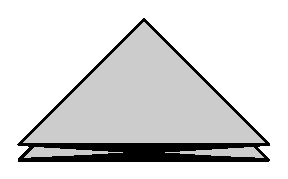
\includegraphics[scale=.98]{src/figure/chap2/fig2-1a.eps}
\end{figure}
\begin{figure}[H]
\centering
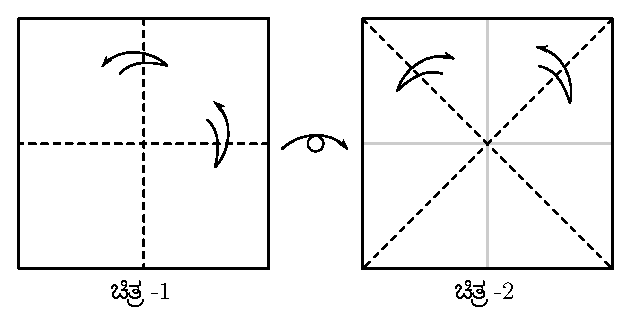
\includegraphics[scale=.98]{src/figure/chap2/fig2-1b.eps}\\
\textbf{1. ಬಣ್ಣದ ಬದಿ ಮೇಲೆ ಇರುವಂತೆ ಚಿತ್ರದಲ್ಲಿ ತೋರಿಸಿದಂತೆ ಮಡಚಿ ತೆಗೆಯಬೇಕು.}\\
\textbf{2. ಕರ್ಣದ ಗುಂಟ ಮಡಚಿ ಬಿಚ್ಚಬೇಕು.}
\end{figure}
\begin{figure}[H]
\centering
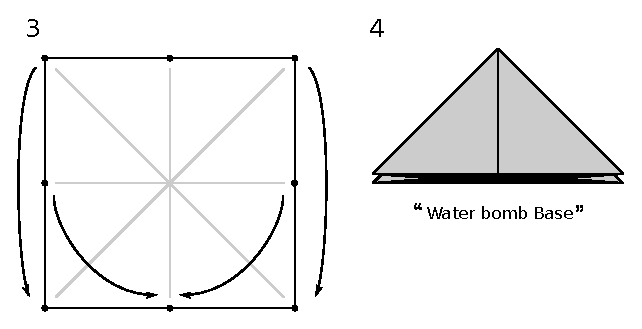
\includegraphics[scale=.98]{src/figure/chap2/fig2-1c.eps}
\end{figure}


\item[{\bf [2]}] \textbf{Preliminary Base: "ಪ್ರಾರಂಭಿಕ ಅಡಿಪಾಯ"}
ಈ ವಿಧಾನವನ್ನು ಪಕ್ಷಿಗಳ, ಕಪ್ಪೆ  ಮತ್ತು `ಲಿಲ್ಲಿ' ಹೂಗಳನ್ನು ತಯಾರಿಸಲು ಅಡಿಪಾಯವಾಗಿದೆ. ಇದು ಹೆಚ್ಚು ಸಾಮಾನ್ಯ ವಿಧಾನವಾಗಿದೆ. 
\begin{figure}[H]
\centering
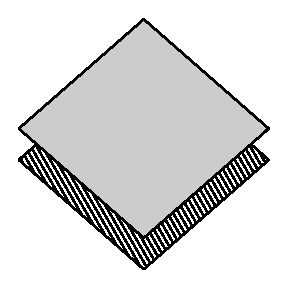
\includegraphics[scale=.98]{src/figure/chap2/fig2-2.eps}
\end{figure}

\textbf{ಮಡಚುವ ಹಂತಗಳು :}
\begin{figure}[H]
\centering
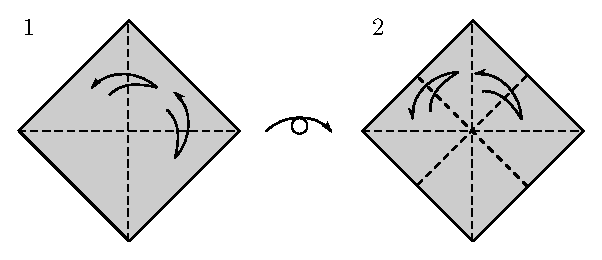
\includegraphics[scale=.98]{src/figure/chap2/fig2-2a.eps}
\end{figure}
\begin{figure}[H]
\centering
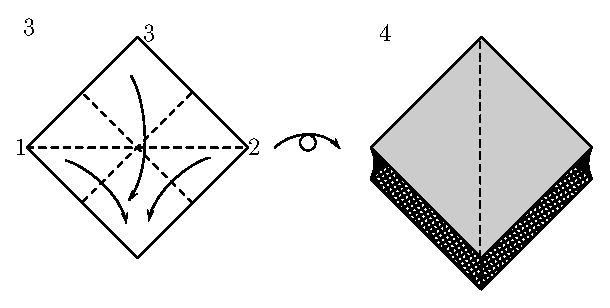
\includegraphics[scale=.98]{src/figure/chap2/fig2-2b.eps}
\end{figure}

\item[{\bf [3]}] \textbf{Frog/Lily Base :} ಇದು "Preliminary base" ವಿಧಾನದಿಂದ ಪ್ರಾರಂಭವಾಗುತ್ತದೆ.
\begin{figure}[H]
\centering
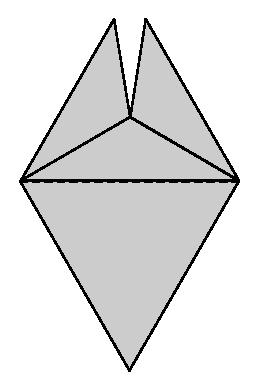
\includegraphics[scale=.98]{src/figure/chap2/fig2-3.eps}
\end{figure}

ಅಂದರೆ, "Preliminary Base" ವಿಧಾನವು ಪೂರ್ಣಗೊಂಡ ನಂತರ ಈ ಮಡಚುವ ಹಂತಗಳು ಪ್ರಾರಂಭವಾಗುತ್ತವೆ.

ಇಲ್ಲಿ ಒಂದು ಬದಿಬಣ್ಣದ ಹಾಗೂ ಇನ್ನೊಂದು ಬದಿ ಬಿಳಿ ಬಣ್ಣವಿರುವ ಕಾಗದವನ್ನು ಚೌರಸ ಆಕಾರದಲ್ಲಿ ತೆಗೆದುಕೊಂಡು ಪ್ರಾರಂಭ ಮಾಡಬೇಕು.

\textbf{ಮಡಚುವ ಹಂತಗಳು :}

\item[{\bf [4]}]

\item[{\bf [5]}]

\item[{\bf [6]}]

\item[{\bf [7]}]

\end{enumerate}
     
 
 
    
